
\chapter{ASPECTOS TEÓRICOS Y REVISIÓN DE LA LITERATURA}
\label{cap:estado_del_arte}

%DESCOMENTAR ESTAS LINEAS SI EL CAPÍTULO TIENE FIGURAS O TABLAS
\addtocontents{lof}{{\bf \noindent Figuras del capítulo \arabic{chapter}}}
\addtocontents{lot}{{\bf \noindent Tablas del capítulo \arabic{chapter}}}

En esta sección se abarcan los aspectos relacionados al conocimiento general para la comprensión del presente trabajo (aspectos teóricos) y la revisión de la literatura asociada al trabajo presentado en esta tesis.
Para realizar un análisis de la Programación Genética aplicada a problemas NP-Completo es necesario conocer la base teórica de ésta. Para ello, se exponen los conceptos fundamentales de la computación evolutiva y la Programación Genética. La sección \ref{cap:aspectos_teoricos} se centra en explicar aquellas partes fundamentales al tema que se trata en esta tesis. De la revisión de la literatura se desprende lo presentado en la sección \ref{cap:rev_literatura}.

\section{Aspectos teóricos}
\label{cap:aspectos_teoricos}


\subsection{Computación Evolutiva}
\label{cap:ce}

A lo largo de la historia, la adaptabilidad de un organismo a un medio en constante variación ha sido la clave para la supervivencia y la evolución (Darwin 1968). Así nace la computación evolutiva (CE), cuyo principio  propone el mismo concepto de supervivencia y transformacion.

Los acontecimientos a los que un organismo se ve sometido conforman la selección que el medio impone sobre éste, y junto a su comportamiento determinan la adaptabilidad del individuo frente a la demanda variable a la cual es expuesto, siendo capaz incluso de encontrar las maneras mas extraordinarias para lograr su objetivo.

Se considera entonces que la evolucion consta de dos fases o etapas:los acontecimientos o variables aleatorias de los organismos y su posterior selección.

Los principios de la CE y sus algoritmos de optimización son la selección impuesta sobre una población inicial de individuos cuyos problemas son creados a partir de soluciones obtenidas al azar o con conocimiento del asunto en cuestión. El resultado de la selección determina una función objetivo (\textit{fitness}), cuyo proceso reiterarivo concluye en generaciones donde quedan los individuos mejor catalogados mediante la reproducción,la selección, cruzamiento y mutación.

La reproducción supone la transferencia del código genético de cada individuo a su descendencia, donde la capacidad reproductiva de las especies es enorme y el número de individuos podría incrementarse exponencialmente si todos sus individuos se pudieran reproducir con éxito simultáneamente, es por eso que existe una probabilidad de que la reproducción se lleve a cabo de forma exitosa. La mutación sucede debido a que los errores en la replicación durante el proceso de transferencia de información genética son inevitables, además de ser necesario incluir variabilidad en las especies. La selección es el resultado de la reproducción de las especies en un medio de competencia dentro de un espacio físico finito donde no hay espacio o recursos para todos y quienes sobreviven son los más aptos.



En la Figura \ref{fig:computacion_evol} se muestra la estructura general de la computación evolutiva, donde se destacan los componentes más importantes de ésta. Estos componentes son: representación (definición de individuos), función de evaluación (o función de \textit{fitness}), población, operadores de variación, cruzamiento, mutación y mecanismo de supervivencia (selección).

\begingroup
    \centering
    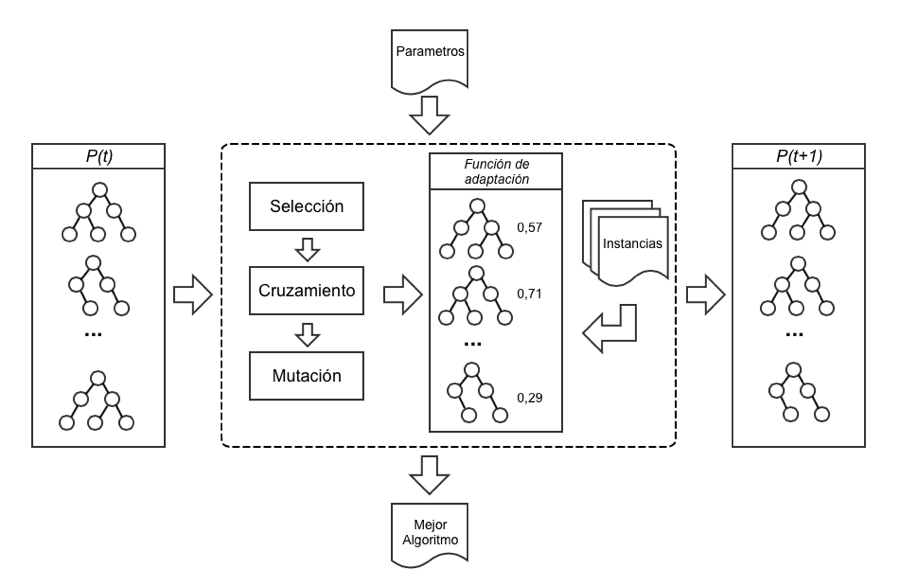
\includegraphics[width=14cm]{images/cap2/computacion_evol2.png}
    \captionof{figure}{Estructura general de la computación evolutiva \citep{contreras_2013}.}\label{fig:computacion_evol}
\endgroup

Los componentes principales para la CE son:
\paragraph{Representación} es una representación del problema a tratar en el mundo real, esto quiere decir que debe existir coherencia entre el espacio de solución a recorrer y el problema en si, para posteriormente poder interpretar la solución producida por la evolución.

\paragraph{Población} Son los individuos que se encuentran en una generación. Se les llama individuos a posibles candidatos que pueden dar solución al problema que se quiere resolver. La población compone la unidad de evolución, donde los individuos se mantienen estáticos, mientas que la población va cambiando.

\paragraph{Inicialización} El objetivo es generar la población inicial, la cual puede ser de forma aleatoria o utilizando alguna heurística. Generalmente,se utiliza la generación aleatória, ya que es la propia CE la que se encargará de mejorar a los individuos.

\paragraph{Función de mejora o {\it fitness}} Es la encargada de medir la aptitud de un individuo de la población (poli et. al 2008). Esta función permite discriminar quienes son los individuos que pasarán a las siguientes generaciones y quiénes no. Es así, dependiendo del problema, la evolución toma una tendencia de maximizar o minimizar, y va guía a generar buenas soluciones.

\paragraph{Operadores de variación} Los operadores permiten generar nuevos individuos a la población a partir de los ya existentes. Su objetivo principal es recorrer nuevas y mejores soluciones no producidas en las generaciones anteriores, con el fin de resolver el problema planteado de la mejor forma.

Los operadores clasicos se destacan tres: cruzamiento, mutación y selección (Falkenauer,1998).
\paragraph{El cruzamiento} Es una operación binaria que permite el intercambio de material entre dos individuos, teniendo como resultados, dos nuevos individuos con información híbrida en cada uno.

\paragraph{La mutación} Opera sobre un individuo, y se aplica para generar diversidad de población.

\paragraph{La selección} Se encarga de obtener la cantidad de los mejores individuos que sobrevivirán al proceso.

\paragraph{Criterio de parada}: Los criterios de parada se pueden diferenciar en dos casos. El primero es conocer el valor óptimo de la solución y que éste sea alcanzado. El segundo puede ser que se han acabado los recursos tales como el máximo tiempo de CPU, un periodo de tiempo, no hay variación en la población, etc. Dentro de la computación evolutiva, existen diversos métodos que utilizan este concepto de una forma más específica de acuerdo a su representación. En el artículo \citep{kouchakpour_2009} se presenta una de las clasificaciones, que se pueden realizar de las variantes de CE. Ésta puede ser vista en la Figura \ref{fig:metodosCE}.

\begingroup
    \centering
    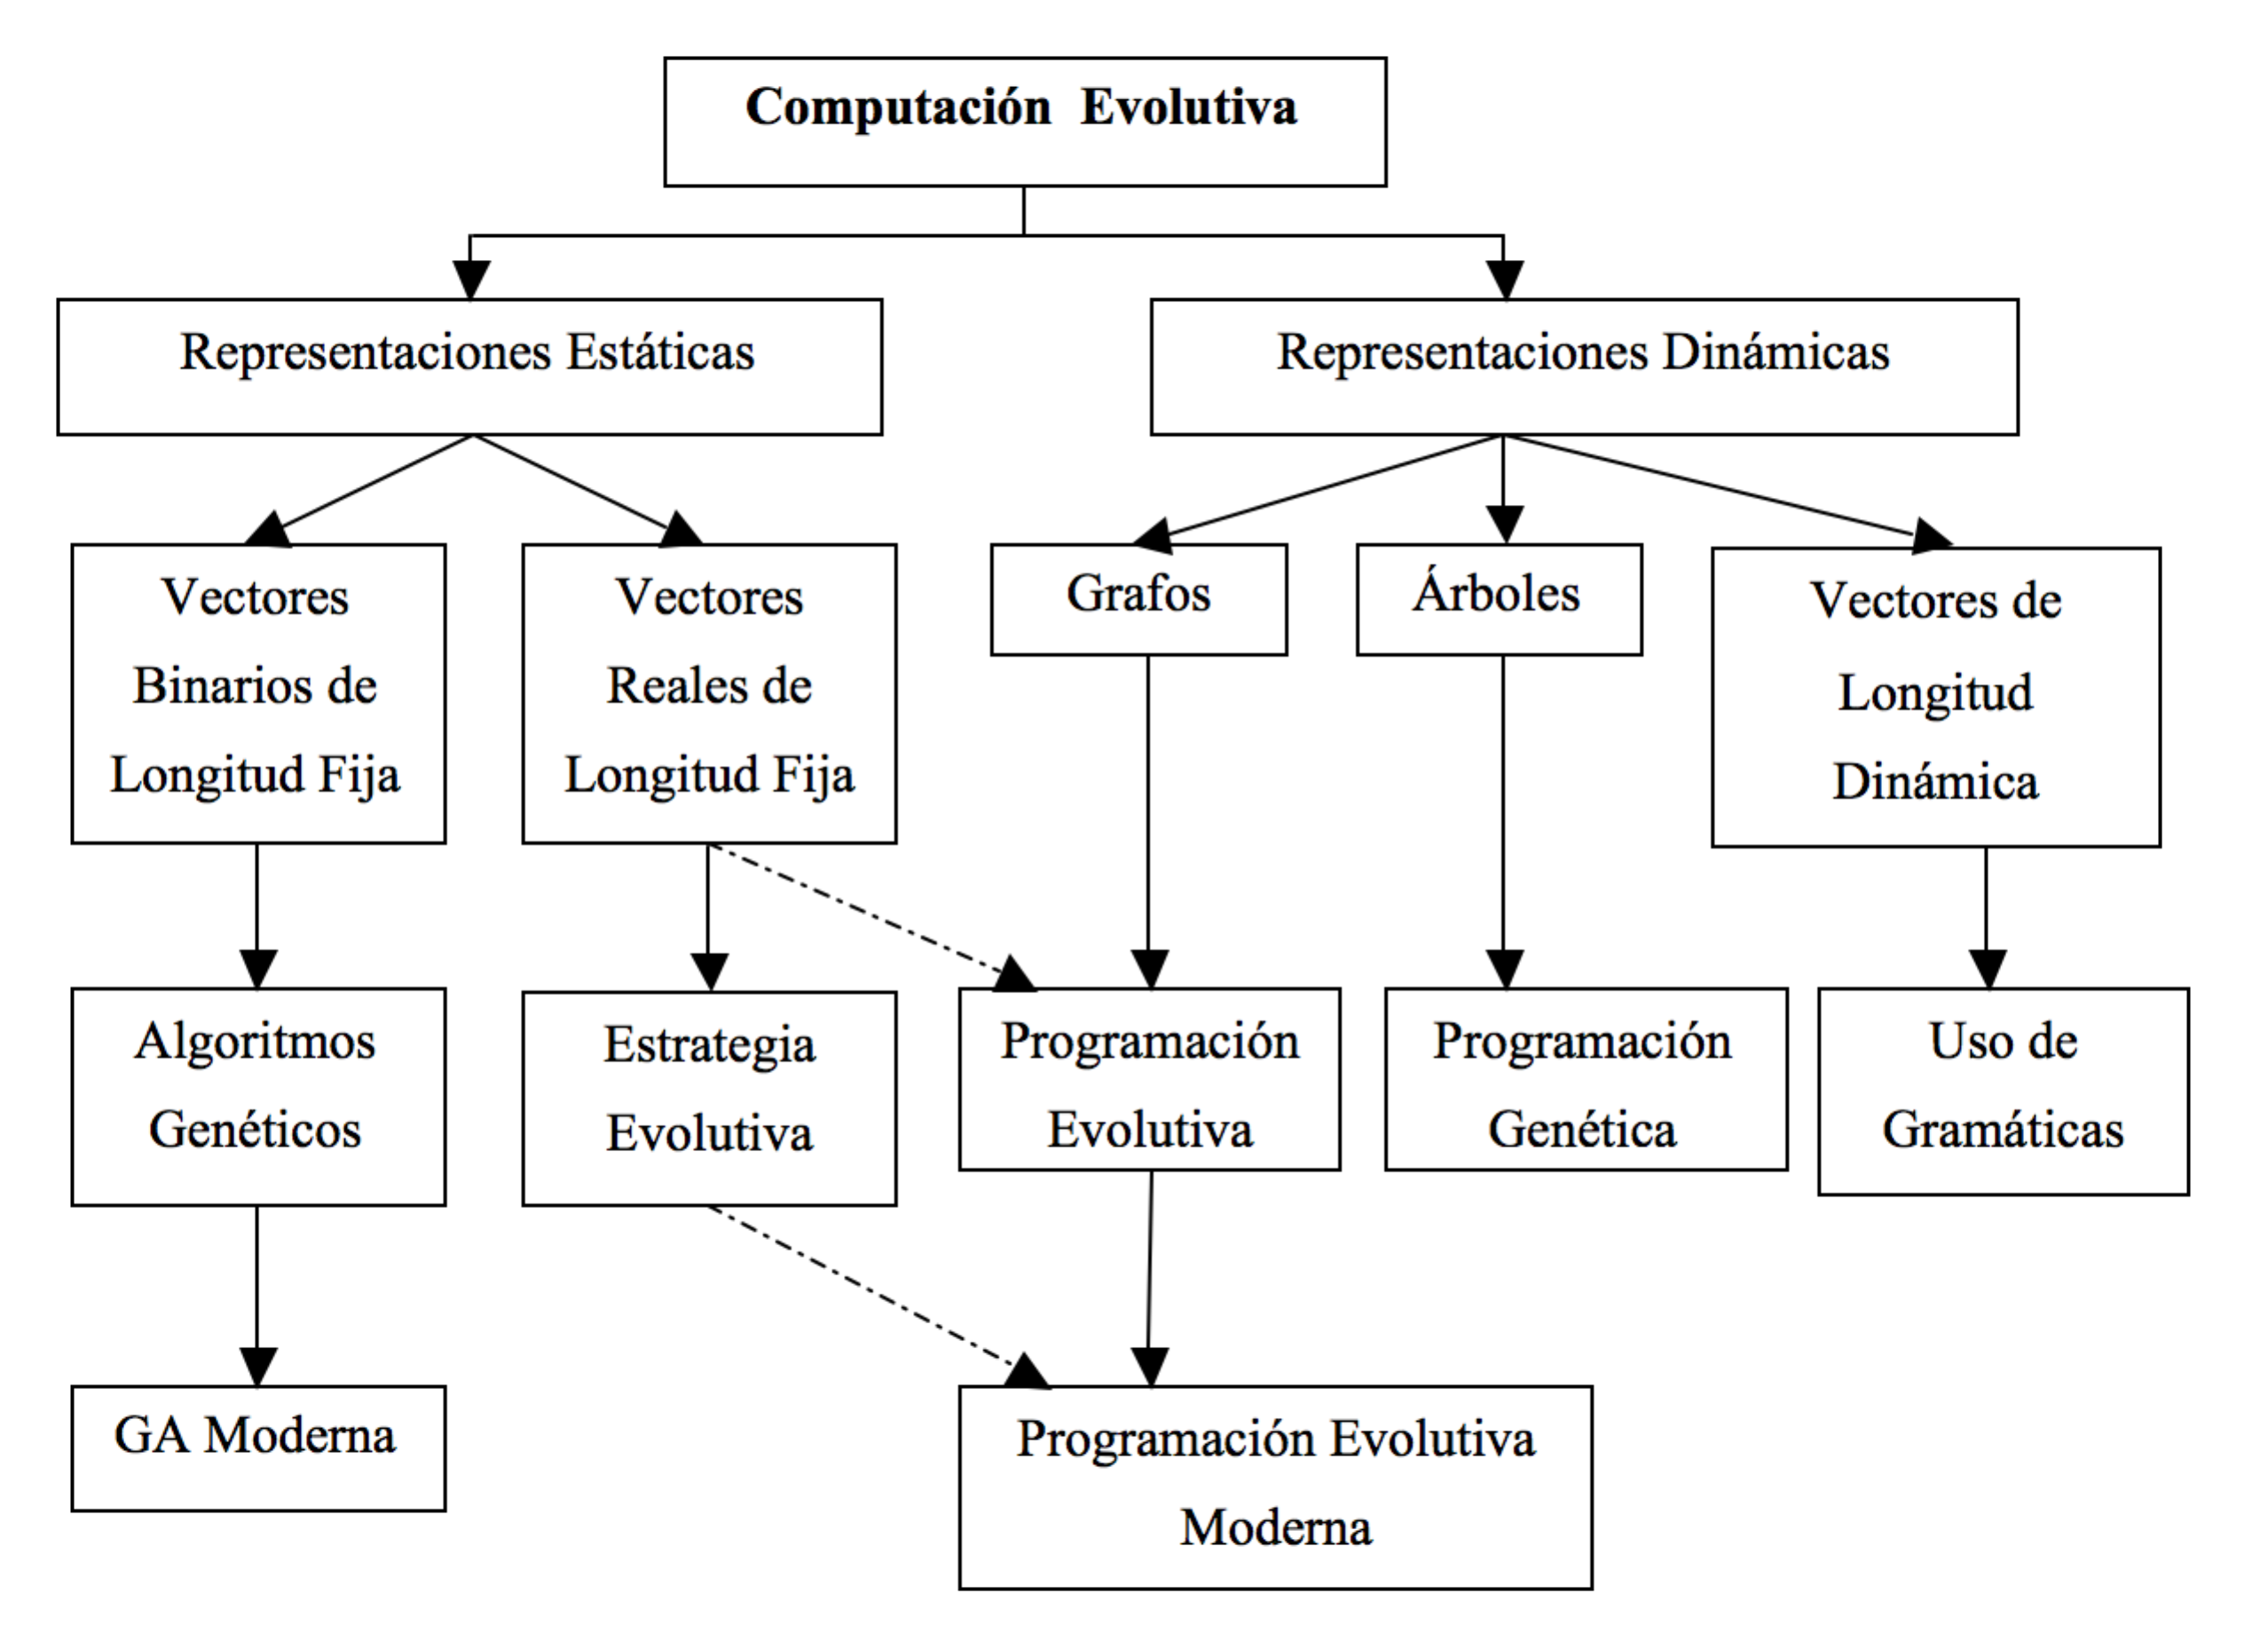
\includegraphics[width=14cm]{images/cap2/metodosCE.png}
    \captionof{figure}{Métodos de la CE basados en el tipo de representación \citep{kouchakpour_2009}.}\label{fig:metodosCE}
\endgroup

\subsection{Programación Genética}
\label{cap:pg}


Una de las tareas más desafiantes de la ciencia de la computación, consiste en que un computador pueda dar solución a problemas sin la necesidad de ser programados de manera explícita. \cite{samuel1959some} declaró:

\textit{¿Cómo pueden los computadores aprender a resolver un problema, sin ser programados explícitamente para ello? En otras palabras, ¿Cómo pueden los computadores hacer lo que tiene que hacer, sin explicitar exactamente cómo tiene que ser hacerlo?}

La Programación Genética (PG) es una técnica de Computación Evolutiva que mediante la generación de código computacional, es capaz de resolver problemas automáticamente, sin la necesidad de que un usuario especifique o conozca la estructura de la solución \citep{poli_2008}. A pesar de no poder garantizar los resultados por ser esencialmente un proceso evolutivo, ha sido muy exitosa y se han encontrado formas inesperadas de resolver problemas \citep{holland_1975}.

En la PG, el proceso evolutivo comienza con una población inicial generada aleatoriamente, la cual es representada por programas computacionales, donde cada individuo es ejecutado y evaluado en virtud de su medida de adaptación frente a un conjunto de casos de prueba propios del problema. Esto se puede apreciar en la figura XX que presenta el diagrama de flujo de los pasos básicos de la PG.


La PG posee tres operadores genéticos, basándose en la selección natural de Darwin, la superviviencia del más apto (operador de selección),la reproducción (operador de cruzamiento) y la mutación. Los operadores se utilizan para crear las nuevas generaciones de individuos que reemplazarán las anteriores \citep{poli_2008}. Generalmente la solución inicial tiene una muy mala calidad, pero algunos individuos serán más aptos que otros. Estas diferencias de adaptación que presenta cada individuo son explotadas a través de las generaciones, y lentamente aquellas caracteristicas individuales que ayudan a resolver el problema, se harán mas comunes en la población. Este funcionamiento se puede ver apreciado en el Algoritmo \ref{alg:programacion_genetica}
\begin{algorithm}[H]
    \begin{algorithmic}[1]
        \STATE {\em Generar Población Inicial aleatoria}
        \WHILE {\em La condición de término sea verdadera}
            \STATE {\em Ejecutar cada programa y determinar su \textit{fitness}}
            \STATE {\em Seleccionar uno o dos individuos-programas de la población para participar en las operaciones genéticas.}
            \STATE {\em Crear nuevo programa mediante la aplicación de las operaciones genéticas}
        \ENDWHILE
    \end{algorithmic}
    \caption{Programación genética}\label{alg:programacion_genetica}
\end{algorithm}



%LISTOOOOOOOOOOOOOOOOOOOOOOO

Para resolver un problema utilizando la PG, \cite{koza_1992} define cinco pasos, los cuales se detallan a continuación:

\begin{itemize}
	\item \textit{Definición del conjunto de terminales}: Permite identificar el conjunto de terminales que van a ser utilizados por los individuos en la población. Los terminales pueden consistir en constantes que representen entradas, sensores o variables de estado, funciones sin argumento, entre otros.

	\item \textit{Definición del conjunto de funciones}: Permite identificar el conjunto de funciones, las cuales corresponden a operaciones elementales posibles, de las que se sospecha puedan intervenir en el cómputo de alguna solución, tales como operaciones aritméticas ($+$,$-$,$*$,$/$), funciones matemáticas ($seno$,$coseno$,$logaritmo$), operaciones booleanas ($and$,$or$,$not$), operaciones condicionales ($if$-$then$-$else$) y funciones que causan iteraciones ($while$,$for$).

	\item \textit{Definición de la medida de aptitud}: Es la encargada de medir la aptitud de los individuos de la población para resolver un problema. La medida de aptitud varía según el problema al que se quiere dar solución. Generalmente se utiliza el error relativo.

	\item \textit{Parámetros de control}: Consiste en escoger los valores de ciertos parámetros que permiten calibrar la evolución. Estos valores pueden ser la probabilidad de cruzamiento, mutación, tipo de selección, entre otros.

	\item \textit{Especificar el criterio de designación de resultado y término de ejecución}: Se puede designar al mejor individuo de todo el proceso de la evolución, a los $k$ mejores individuos de las últimas generaciones u otra alternativa que sea apropiada al problema que se quiere resolver. Para el criterio de término, se puede fijar un número máximo de generaciones o algún equivalente de éxito como un valor de evaluación de desempeño, entre otros.
\end{itemize}



Adicionalmente, para una correcta implementacion de la PG, existen dos propiedades que se deben considerar al momento de construir las funciones y terminales:

\begin{itemize}


\item \textit{Suficiencia}: Las funciones y terminales utilizados deben ser suficientes para representar una solución para el problema \citep{koza_1992}. Si el diseño no es apropiado o suficientemente representativo, la PG no podrá encontrar una solución factible al problema planteado.

\item \textit{Clausura}: Cada función debe ser capaz de manejar de forma adecuada los argumentos que pueda recibir como entrada, estos son los posibles valores retornados por otras función definida en el conjunto y cualquier valor o tipo de dato que sea alcanzable desde el conjunto de terminales \citep{koza_1992}. La clausura no es una propiedad indispensable, en los casos que no se puede garantizar, se debe utilizar alternativas tales como, la eliminación de individuos o la penalización sobre su medida de aptitud cada vez que algún individuo contenga alguna construcción infactible.


% LISTOOOOOOOOOOOOOOOOOOOOOOOOOOOOOOOOOOO

%como entrada, ya sea que provengan de otras funciones definidas o parámetros que pueden alcanzar los terminales definidos.

%	\item Suficiencia del conjunto de funciones y terminales: la propiedad de suficiencia está relacionada con la capacidad de expresar un programa computacional que resuelva un problema planteado en términos de las funciones y terminales definidos para ello \citep{koza_1992}. Cada problema requiere un diseño apropiado, basado en un amplio conocimiento del dominio. En ocasiones, su definición puede llegar a ser muy difícil o virtualmente imposible \citep{koza_1992, poli_2006}.

%	\item Clausura del conjunto de funciones: la clausura es una propiedad deseable para el conjunto de funciones, pero no indispensable, ésta consiste en que cada función debe aceptar como argumentos el resultado . Existen casos donde no es posible garantizar la clausura del conjunto de funciones, en estas situaciones se debe utilizar alternativas tales como, la eliminación de individuos o la penalización sobre su medida de aptitud cada vez que alguno de ellos incorpore en su código alguna construcción infactible.

\end{itemize}


A partir de la última década del siglo $XX$, la PG ha sido considerada como un método "humano competitivo" para la resolución de problemas. Las principales razones de esta clasificación se debe a que la mayoría de los problemas planteados en inteligencia artificial, aprendizaje automático y sistemas adaptativos pueden ser formulados como una búsqueda de programas computacionales, y la técnica de PG entrega una forma satisfactoria de guiar la búsqueda en el espacio de programas computacionales \citep{affenzeller_2001}.

Turing, en el año 1948, advirtió correctamente que una posible aproximación a la inteligencia artificial incluiría un proceso evolutivo, donde un programa computacional (material hereditario) sea sometido a una modificación progresiva (mutación) bajo la dirección de la selección natural \citep{koza_poli_2005}.

Un resultado generado por un método automatizado puede ser clasificado como “humano competitivo”, independiente del hecho de que sea generado de forma automática. Sin embargo, un resultado humanamente competitivo obtenido debe tener un cierto grado de complejidad, es por esto que un resultado generado por un método automatizado que resuelve un \textit{“toy problem”} (por ejemplo, las torres de Hanoi, apilamiento de bloques, caníbales y misioneros), no sería considerado como “humano competitivo”, debido a que la solución no es publicable como un nuevo resultado científico, sólo es de interés porque fue creado de forma automática.

Así, según Koza \citep{koza_2003}, una solución generada automáticamente para un problema es humanamente competitiva si ésta satisface uno o más de los ocho criterios que se muestran en la Tabla \ref{tab:human_comp}.

\begin{table}[ht]
\caption{Criterios para un resultado “humano-competitivo” \citep{koza_2003}.}\label{tab:human_comp}
\small
\centering
\rowcolors{2}{white}{blue!25}
\begin{tabular}{cl}
\hline
{\textbf{Nº}} & \multicolumn{1}{c}{\textbf{Criterio}} \\ \hline

A  & \begin{tabular}[c]{@{}l@{}} El resultado fue patentado como un invento, es una mejora de una invención patentada, \\o podría calificar como una nueva 		invención patentable.   \end{tabular}  \\
B  & \begin{tabular}[c]{@{}l@{}} El resultado es igual o mejor que un resultado científico aceptado y publicado en una \\ revista científica. \end{tabular}  \\
C  & \begin{tabular}[c]{@{}l@{}} El resultado es igual o mejor que un resultado que fue colocado en una base de datos o \\ archivo de resultados y gestionada por un panel internacional de expertos científicos reconocidos. \end{tabular}  \\
D  & \begin{tabular}[c]{@{}l@{}} El resultado es publicable como un nuevo resultado científico, independiente del hecho \\ que fue creado mecánicamente. \end{tabular}  \\
E  & \begin{tabular}[c]{@{}l@{}} El resultado es igual o mejor que un resultado reciente de un problema que ha tenido \\ sucesivos resultados cada
	vez mejores.  \end{tabular}                  \\
F  & \begin{tabular}[c]{@{}l@{}} El resultado es igual o mejor que un resultado que se consideró un logro en su campo \\ en el momento en que fue descubierto.	\end{tabular}                  \\
G  & \begin{tabular}[c]{@{}l@{}} El resultado soluciona un problema de dificultad indiscutible en su campo.	\end{tabular}                  \\
H  & \begin{tabular}[c]{@{}l@{}} El resultado está entre los mejores o gana una competencia regulada que incluye \\ participantes humanos.	\end{tabular}  \\
\hline
\end{tabular}
%\caption*{(Elaboración propia, 2015)}
\end{table}

La obtención de resultados humanamente competitivos ha incentivado el crecimiento del campo de la computación genética y evolutiva, esto se debe a que la obtención de estos resultados depende del progreso, desarrollo y perfeccionamiento de los métodos de búsqueda genéticos y evolutivos. No obstante, a medida que resultados humanamente competitivos sean generados, irán apareciendo problemas más desafiantes.

\section{Revisión de la literatura}
\label{cap:rev_literatura}

\subsection{Generación automática de algoritmos}
La generación automática de algoritmos (GAA) ha sido utilizada los últimos años para resolver distintos problemas de optimización combinatoria. En este proceso, los algoritmos pueden ser generados mediante el uso de hiper-heurísticas que poseen estructuras que permiten ser interpretadas como algoritmos. Se pueden encontrar varios trabajos que utilizan la PG para realizar la GAA \citep{contreras_2013, drake_2014, parada_2015}.

El proceso para diseñar hiper-heurísticas que permitan obtener una solución a un problema de optimización combinatoria consta de tres fases \citep{alinia_2012}. La primera corresponde a la formulación matemática del problema. La segunda fase es el diseño de heurísticas de bajo nivel que permitan entregar una solución apróximada al problema. Y la tercera fase procesa, por medio de una hiper-heurística, diferentes combinaciones de las heurísticas definidas en la segunda fase. El proceso de selección de heurísticas se puede realizar a través de métodos de adaptación que buscan los mejores resultados en el espacio de soluciones de acuerdo con una medida de rendimiento \citep{parada_2015}.

%El desarrollo de la generación automática de algoritmos (GAA) es un tema que ha tomado mayor importancia en los últimos años. En este proceso, algoritmos pueden ser generador por hiper-heurísticas que poseen estructuras que pueden ser interpretadas como algoritmos. En la literatura existen varios trabajos que utilizan la PG para realizar la GAA \citep{contreras_2013, drake_2014, parada_2015}.

%El diseño de hiper-heurísticas para problemas de optimización combinatoria es un proceso que consta de tres etapas \citep{alinia_2012}. La primera de ellas es el problema a resolver, definido por su formulación matemática. La segunda consiste en heurísticas de bajo nivel que permiten dar solución al problema de forma aproximada. Finalmente, la tercera permite procesar por medio de una hiper-heurística diferentes combinaciones de las heurísticas definidas en la etapa 2. Por otra parte, la correcta selección de heurísticas es determinada en el presente trabajo, debido a que la selección de heurísticas o combinación de éstas es un problema de optimización combinatoria.

%El proceso de selección heurística se puede realizar a través de métodos de adaptación o meta-heurísticas que buscan los mejores resultados en el espacio de soluciones. El proceso de búsqueda encuentra una heurística que ofrece la mejor opción en cada movimiento de acuerdo con alguna medida de rendimiento \citep{parada_2015}.

\subsection{Heurísticas y meta-heurísticas}

En la actualidad, para resolver problemas computacionalmente complejos es necesario desarrollar algoritmos más avanzados. Los algoritmos exactos suelen requerir una gran cantidad de tiempo debido al tamaño del espacio de soluciones factibles. Para solucionar éste problema, han sido desarrollados los algoritmos aproximados, que, mediante el uso de heurísticas y meta-heurísticas, permiten encontrar soluciones que se acercan a una mejor solución. Los algoritmos heurísticos utilizan funciones especiales, las que están diseñadas para encontrar el espacio de soluciones de forma inteligente.


%Hoy en día los computadores son utilizados para resolver problemas computacionalmente complejos. Para resolver estos problemas es necesario desarrollar algoritmos más avanzados. Los algoritmos exactos para resolver estos problemas pueden requerir un tiempo inaceptable dado el espacio de búsqueda de soluciones factibles. Para hacer que un algoritmo de búsqueda obtenga soluciones en un tiempo aceptable, se han desarrollado algoritmos aproximados. Este tipo de algoritmo ocupa heurísticas y meta-heurísticas para encontrar las soluciones. Los algoritmos heurísticos utilizan las funciones especiales, diseñadas para averiguar el espacio solución de forma inteligente.

En la Figura \ref{fig:tax_opt} se muestra la clasificación de diferentes problemas de optimización, los cuales están divididos en dos categorías: algoritmos exactos y algoritmos aproximados \citep{desale_2015}.

\begin{figure}[H]
%\begingroup
    \centering
    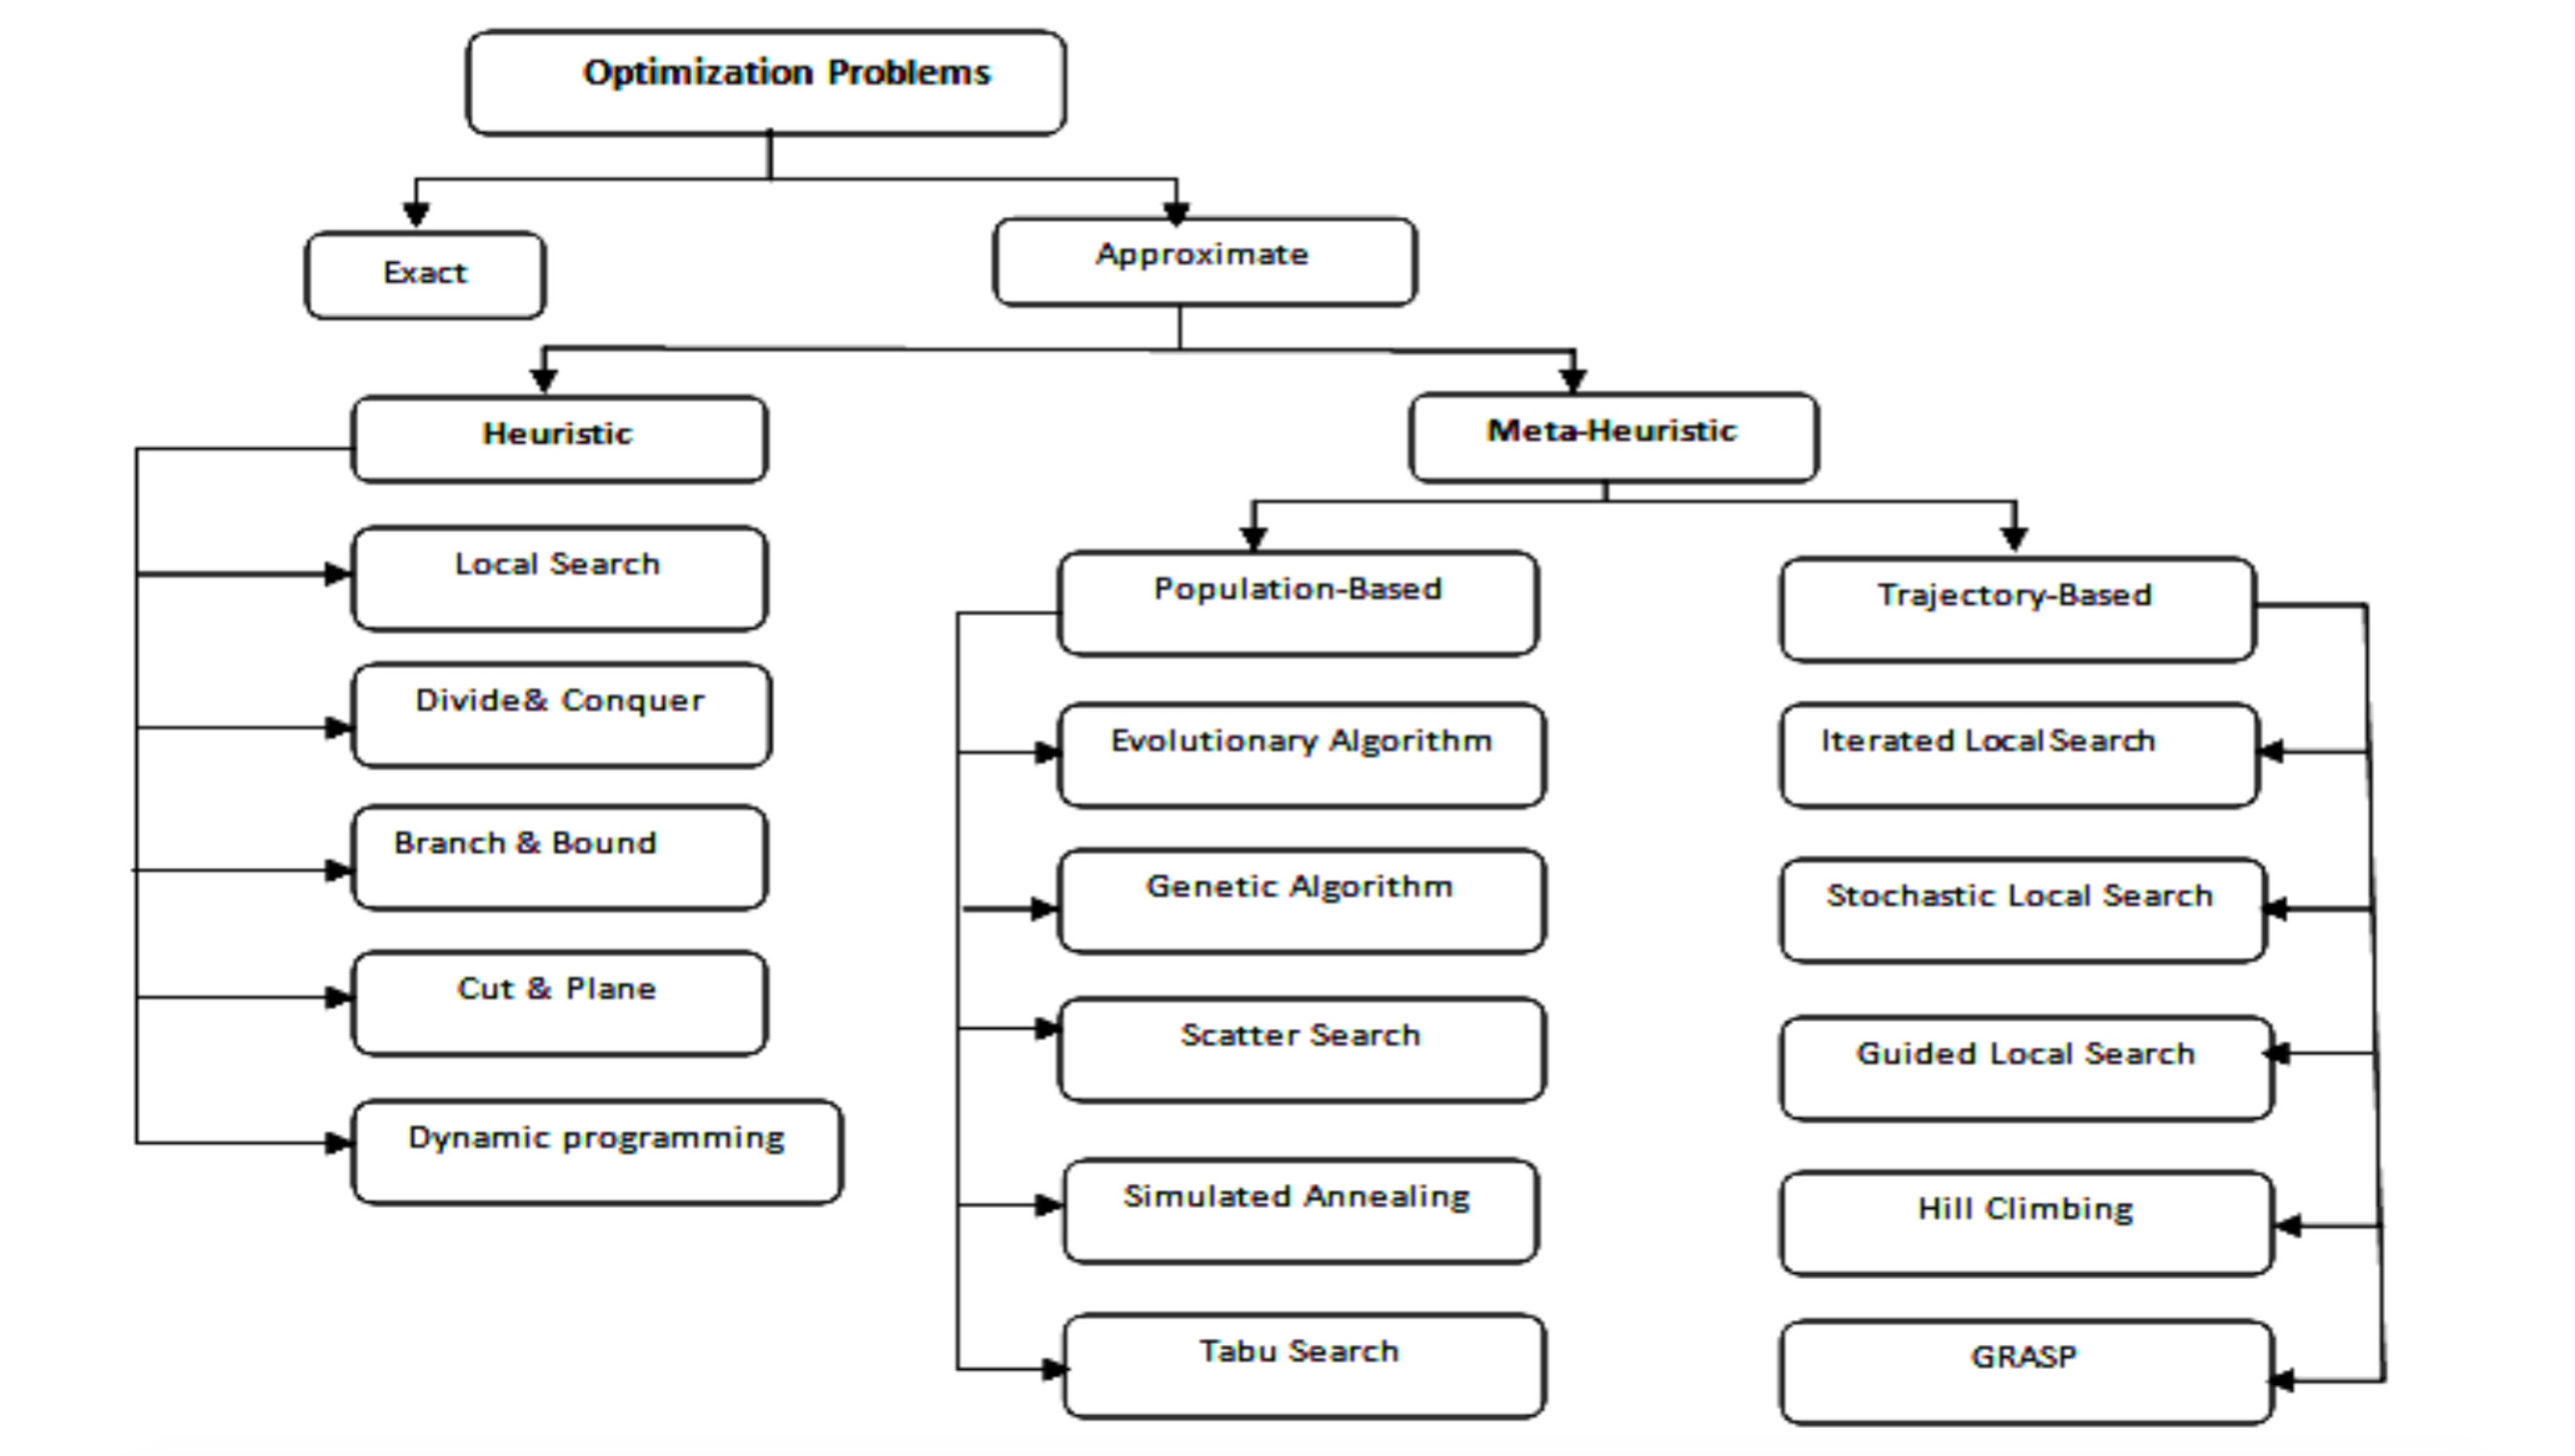
\includegraphics[width=16cm]{images/cap2/tax_opt.png}
    \captionof{figure}{Métodos utilizados para resolver problemas de optimización \citep{desale_2015}.}\label{fig:tax_opt}
%\endgroup
\end{figure}


Los algoritmos meta-heurísticos son el proceso de generación iterativo que guía una heurística para explorar y explotar el espacio de búsqueda.

Las heurísticas y meta-heurísticas son utilizadas para encontrar una solución óptima en un espacio de búsqueda discreto en problemas de optimización combinatoria. Un ejemplo es el problema del vendedor viajero, donde la búsqueda del espacio de soluciones factibles crece exponencialmente en función del tamaño del problema aumenta, lo que hace inviable la realización de una búsqueda exhaustiva de la solución óptima \citep{desale_2015}.

%Heurística y meta-heurísticas se utilizan para la optimización combinatoria en la que se busca una solución óptima en un espacio de búsqueda discreto. Un problema de ejemplo es el problema del vendedor viajero, donde la búsqueda del espacio de soluciones factibles crece exponencialmente a medida que el tamaño de los problemas aumenta, lo que hace inviable una búsqueda exhaustiva de la solución óptima \citep{desale_2015}.

\subsection{Hiper-heurísticas}

El término de hiper-heurística fue utilizado por primera vez en el año 2000 para lograr describir una heurística que escoge heurísticas en el contexto de la optimización combinatoria. Mientras que la automatización del diseño de heurísticas se remonta a la década de 1960. La definición de hiper-heurísticas  se refiere a un método de búsqueda o mecanismo que permite seleccionar o construír la heurística que resuelve problemas de búsqueda de cálculo de aprendizaje. Se pueden diferenciar dos categorías: la selección de heurísticas y la generación de las mismas. La características de las hiper-heurísticas es que operan en un espacio de búsqueda de una heurística y no directamente en el espacio de búsqueda de soluciones del problema en cuestión \citep{burke_2013}.

El proceso para generar algoritmos en forma automática puede entenderse como una hiper-heurística, o como una metodología, cuando la generación automática de algoritmos se realiza mediante el uso de la programación genética y definición del proceso evolutivo. En ambos casos existen elementos comunes que permiten generar artefactos que resuelvan el problema en estudio, un proceso de mejora guiado por una función objetivo, entre otros. El proceso de generación de algoritmos busca obtener una estructura que se expresa mediante un árbol sintáctico y luego se decodifica para su posterior comprensión e interpretación. El objetivo del proceso es poder extraer conocimiento nuevo para recrear los algoritmos existentes en la literatura. Además, la GAA permite generar algoritmos que contemplen el uso de las mejores heurísticas o algoritmos existentes para el problema. Mientras que las hiper-heurísticas son utilizadas para resolver en forma eficiente el problema sin necesidad de realizar una interpretación del resultado obtenido \citep{burke_2013}.

%El término hiper-heurística es relativamente nuevo; fue utilizado por primera vez en el año 2000 para describir una heurística que escoge una heurística en el contexto de la optimización combinatoria. Sin embargo, la idea de automatizar el diseño de la heurística no es nueva; este se remonta a la década de 1960. La definición de hiper-heurística se ha ampliado recientemente para referirse a un método de búsqueda o mecanismo para seleccionar o generar la heurística para resolver problemas de búsqueda de cálculo de aprendizaje. Dos categorías principales de hiper-heurística pueden ser considerados: la selección de heurística y la generación de heurística. La característica distintiva de hiper-heurística es que operan en un espacio de búsqueda de una heurística (o componentes heurísticos) en lugar de hacerlo directamente en el espacio de búsqueda de soluciones para el problema que se está abordando \citep{burke_2013}.

%El proceso de generación automática de algoritmos puede ser visto como una metodología o como una hiper-heurística cuando la generación automática de algoritmos se realiza a través de la programación genética y siguiendo los pasos canónicos, que consiste en la generación de funciones y terminales, y definición del proceso evolutivo. Ambas tienen elementos en común que permiten generar dispositivos, aparatos o algoritmos que resuelvan el problema en estudio, un proceso gradual de mejora guiado por una función objetivo, etc. La diferencia entre ambas es que un proceso de generación de algoritmos busca generar una estructura que se expresa mediante un árbol sintáctico y posteriormente se descodifica su correspondiente pseudo código para que sea perfectamente comprensible e interpretable por el ser humano. El objetivo de realizar la generación de esta forma es que el ser humano pueda extraer conocimiento nuevo para recrear los algoritmos existentes en la literatura. También la GAA permite generar algoritmos que contengan las mejores heurísticas o algoritmos disponibles para el problema que provienen de la literatura. A diferencia de ello, las hiper-heurísticas son ocupadas para resolver eficientemente el problema sin que sea necesario realizar una interpretación de la estructura o del código obtenidos. Asimismo, las hiper-heurísticas que se han experimentado hasta ahora utilizan distintas formas de obtener las estructuras de los problemas de optimización general \citep{burke_2013}.



\subsection{Instancias}
\label{cap:instancias}


-------------------------((PENDIENTE))------------------------

Durante los últimos años, se han desarrollado cada vez algoritmos más sofisticados para problemas de optimización. Estos algoritmos incluyen distintos métodos o técnicas, los que son sometidas a estudios experimentales que tienen por objetivo determinar que algoritmo obtiene un mejor rendimiento, usualmente éstos se basan en conjuntos de instancias públicas. El teorema de \textit{no free lunch} (NFL) dice que no existe un algoritmo que sea superior a todos los demás algoritmos en todas las instancias posibles de un problema. Si un algoritmo se declarase como mejor que otro conjunto de algoritmos, entonces es posible esperar que existan instancias que aún no han sido probadas. Es por esto que una de las claves para poder realizar un correcto estudio es caracterizar las instancias del problema de acuerdo a su dificultad y al espacio de soluciones que las representa \citep{smith_2012}.

Las características más sencillas de una instancia para un problema de optimización son las que se definen como parte de la sub-clase de la instancia: características como el número de variables y restricciones, o si las matrices que almacenan los parámetros son simétricas, etc.

Para el PVV, una forma de clasificar las instancias es mediante la distribución de costos que posee (distancias entre los nodos o ciudades), donde se muestra el número de valores distintos que poseen las distancias \citep{smith_2012}. Las instancias a utilizar para este problema, son obtenidas de la TSPLib \citep{reinelt_1991}. Esta librería contiene instancias ampliamente utilizadas en la literatura, las que en su totalidad cuentan con su valor óptimo y, en algunos casos, con una posible solución.

La clasificación para las instancias del PM-01 ha sido altamente estudiada por Pisinger. La clasificación más común es la realizada en base a la relación que poseen el beneficio y peso de cada uno de los ítems de una instancia, donde propone una variedad de grupos. Estos grupos poseen características desde una igualdad beneficio-peso hasta grupos donde no existe relación alguna entre éstos. Adicionalmente, es propuesta una clasificación con relación a las magnitudes de los valores que pueden alcanzar los elementos \citep{pisinger_2005}. Las instancias a utilizar para este problema son las utilizadas por Pisinger \citep{pisinger_2005}.

\subsection{Revisión de la literatura para PCMR}



El PCMR, que pertenece a la clase NP-Hard \citep{joksch1966shortest}, consiste en encontrar un camino o cadena de aristas $P_{cad}$ desde un vértice inicial $v_s$ perteneciente a \emph{V}, a un vértice final $v_e$ también perteneciente a \emph{V}, que minimice el costo total de aristas en $P_{cad}$ y que además la suma de los recursos o pesos de cada aristas no exceda un máximo de recurso a consumir denotado \emph{W} \citep{dumitrescu2001algorithms}. Su formulación matemática es la siguiente:
%Sea \emph{G =(V,A)}, un grafo sin ciclos y dirigido, donde \emph{V=\{1,2...n\}}  es un conjunto de vértices, $|V|=n$ y \emph{A} es un conjunto de arcos tal que $A= \{(i,j):i,j \in V, i \neq j\}$. Cada arco \emph{(i,j)} perteneciente a \emph{A} posee un costo no negativos $C_{i,j}$ y posee además un recurso o peso no negativos $W_{i,j}$.

%Teniendo en cuenta estas definiciones, el problema CSP se puede formular como un problema de programación entera binaria de la siguiente manera:

\begin{equation}
min \sum_{i,j \in A}^{}{c_{ij}x_{ij}}
\end{equation}

\begin{equation}
sujeto  \sum_{j:(i,j) \in A }^{}{x_{ij}} - \sum_{k:(k,i) \in A}^{}{x_{ki}} = \begin{cases}
      1              & \mbox{si } i= v_s   \\
      0 			 & \mbox{si } i= 2,..... n-1 \\
      -1 			 & \mbox{si } i= v_e
   \end{cases}
\end{equation}

\begin{equation}
\sum_{i,j: (i,j) \in A}^{}{w_{ij}x_{ij}} \leq W
\end{equation}

\begin{equation}
x_{ij} /x_{ij} \in  \left \{0,1 \right \} , (i,j)  \in A
\end{equation}

%La variable $x_{ij}$ son variables binarias que se encuentran asociadas a cada arco $(i,j)$. Si el arco está incluido en la ruta óptima, entonces $x_{ij}=1$, en caso contrario $x_{ij}=0$. El parámetro $W$ representa el valor máximo del peso a no sobrepasar para la suma de los pesos de las aristas $w_{ij}$, y $c_{ij}$ es el costo asociado. De ésta forma,
%La ecuación (2.1) se plantea el problema de minimización, donde se suman todos los costos considerados en el camino,
La ecuación (2.2) da a conocer que debe ser una cadena conexa desde el nodo inicial $v_s$ a $v_e$, y la ecuación (2.3) plantea que la suma de los pesos de las aristas consideradas en el camino no debe sobrepasar el peso $W$ \citep{santos2007improved}.


%El problema del camino mínimo con restricción (PCMR), que pertenece a la clase NP-Hard \citep{joksch1966shortest}, consiste en encontrar la ruta más corta entre dos puntos, pero no debe sobrepasar un peso $W$ también asociado al camino. Existen diversas aplicaciones prácticas en el mundo real para el CSP, como el problema de ruteo de buses \citep{cho2007intermodal}, gestión de aeronaves \citep{zabarankin2002optimal}, usos militares \citep{royset2009routing}, entre otros. La formulación matemática es la siguiente:


%\begin{eqnarray}
%\min \sum_{i, j \in A}^{m} c_{ij}x_{ij}
%\end{eqnarray}
%Sujeto a
%\begin{eqnarray}
%\sum_{j : (i, j) \in A}^{m} x_{ij} - \sum_{k : (k, i) \in A}^{m} x_{ki}
%&=&
%\left\{
%\begin{array}{rrl}
%  1   & si  & i = s\\
%  0   & si  & i = 2, \ldots, m - 1\\
%  -1  & si  & i = t
%\end{array}
%\right.\\
%\sum_{i, j: (i, j) \in A}^{m} w_{ij}x_{ij} &\leq& W\label{form:2_3}\\
%x_{ij} \in \{0, 1\}&&  (i, j) \in A
%\end{eqnarray}
%La ecuación \ref{form:2_1} verifica que sea un camino conexo desde el nodo inicial $s$ al nodo final $t$. Mientras que la ecuación \ref{form:2_2} da a conocer el dominio de $x_{ij}$. La ecuación \ref{form:2_3} plantea que la suma de los pesos de las aristas consideradas en el camino no debe sobrepasar el peso $W$.

Las estrategias utilizadas para el PCMR se pueden clasificar en dos categorías principales, programación dinámica y relajación lagrangiana. Los métodos basados en la programación dinámica también se conocen como \textit{label setting} o \textit{label correcting}. Una de las características de este tipo de algoritmos es que en instancias de tamaño razonable, pueden ser muy veloces; sin embargo, para redes que pueden tomar dimensiones muy grandes podrían dejar de ser una buena alternativa, esto debido a que el número de etiquetas que deben ser almacenadas  puede ser muy grandes y como consecuencia pueden ser imposibles de manejar.

Uno de los primeros algoritmos pertenecientes a esta categoría fue propuesto por \cite{joksch1966shortest}, el cual fue extendido por \cite{dumitrescu2003improved}, comparandse con tres algoritmos \cite{dumitrescu2001algorithms,hassin1992approximation,lorenz2001simple} a los que supera en término de tiempo computacional y requisitos de memoria. Los autores afirman también que la integración entre las técnicas de relajación langrageana y pre-procesamiento podrían mejorar el tiempo de ejecución.

Posteriormente, se presentan un enfoque de etapas para abordar el camino mínimo con un conjunto de restricciones o recursos (PCMG) \cite{zhu2012three}. Para ello se propone un algoritmo pseudopolinomial llamado TSA en tres etapas: la primera es un pre-procesamiento de las instancias reduciendo los arcos y los vértices, disminuyendo el espacio de búsqueda, el segundo es un proceso de \textit{setup} para transformar el PCMG a un PCM, el tercero es un procesamiento iterativo de búsqueda. El TSA es comparado con CPLEX (REFERENCIA FALTANTE) y con el algoritmo \textit{label setting} \citep{dumitrescu2003improved} para cuatro tipos distintos de problemas, mostrando abordar de forma eficaz los casos de prueba, pero el tiempo de ejecición aumenta a medida que los problemas se van haciendo más grandes en cantidad de nodos y conjunto de recursos.

El segundo enfoque para dar solución al PCMR se basa en el uso de la relajación lagrangiana para resolver la formulación de programación entera del problema. La eficiencia de este enfoque se basa en la eficacia de los algoritmos de ruta más corta sin restricciones subyacentes. Un algoritmo exacto para el problema PCMR basado en relajación Langragiana al cual es denotado como LRA (lagrangian relaxation algorithm)\citep{santos2007improved}. El LRA se compara con métodos de \textit{k-shortest path} y con métodos de relajación langragiana, ambos introducidos por \cite{handler1980dual}. Los resultados de estas pruebas indican que el LRA puede abordar grandes problemas teniendo ventajas sobre los otros métodos en términos de tiempo computacional y en el uso de memoria. Sin embargo, los autores comparan su algoritmo sólo con \cite{handler1980dual}, y no con los algoritmos mejorados de \citep{dumitrescu2003improved}.

Luego, se expone un nuevo algoritmo basado en relajaciones Langragianas con enumeraciones de caminos mínimos al cual denominan LRE (\textit{lagrangian relaxation and enumeration}), el cual se sostiene en técnicas de pre-procesamientos \citep{carlyle2008lagrangian}. En el trabajo se utiliza cuatro grupos de casos de prueba y se compara con el \textit{label setting} \citep{dumitrescu2003improved}, donde el LRE resuelve hasta el doble de casos que el \textit{label setting} en un tiempo de 30 minutos. Sin embargo, existen casos que el LRE no supera al \textit{label setting}, debido a la existencia de grandes distancias entre las cotas inferiores y superiores, teniendo un tiempo de ejecución más prolongado. Mientras que en el 2009, se da a conocer un enfoque Langragiano dual al cual se denomina eliminación agresiva de costos (AEE) \citep{muhandiramge2009simultaneous}. Consiste en una versión modificada del algoritmo expuesto por \citep{carlyle2008lagrangian}. AEE se compone de dos etapas principales: primero relaja el problema con métodos duales Langragianos con iteraciones, todo ello mediante la restricción de pesos con pasos de pre-procesamiento, después, aborda el problema basándose en las cotas de la red ya reducida por el pre-procesamiento. Se da a conocer que se podrían mejorar los resultados siempre y cuando se encuentren buenos parámetros iniciales, como las cotas iniciales o múltiplos iniciales, lo cual no se investigó en el artículo científico.

Posteriormente, se propone un método exacto llamado \textit{Pulse} que maneja redes de gran escala para el problema del PCMR \citep{lozano2013exact}, encontrando mejores resultados en los 180 casos propuestos en la literatura, respecto al algoritmo de \cite{santos2007improved}, logrando aceleraciones de hasta 60 veces. También supera favorablemente al algoritmo propuesto por \cite{dumitrescu2003improved}, logrando aceleraciones de hasta 900 veces con las dos series de casos propuestos para el problema.

En uno de los últimos trabajos se propone un modelo mejorado llamado Ameba para abordar el problema del PCMR \citep{zhang2013adaptive}. El modelo Ameba consiste en un conjunto de tubos interconectados que emulan a esta bacteria, y que posteriormente, construyen un modelo matemático \citep{nakagaki2001path}. Para resolver el problema, adaptan el modelo de Ameba al problema de PCMR y después integran un proceso de relajación Langragiana. Se afirma que el método es capaz de abordar problemas del PCMR, pero sólo con los casos de selección de rutas en redes de transporte y de computadora propuestos en su investigación.



\subsection{Revisión de la literatura para PACMG}
\label{cap:rev_lit_pvv}



El PACMG, que pertenece a la clase NP-Hard \citep{dror2000generalized}, consiste en un grafo no dirigido cuyos nodos son divididos en $k$ clúster, para determinar un árbol de cobertura de costo mínimo que incluya sólo un vértice de cada cluster. Se define matemáticamente por un grafo no dirigido $G = (V,E)$ de $n$ vértices, $m$ aristas y $ V_{1},..., V_{k}$ una división de $V$ en $k$  subconjuntos (clúster), donde, $ V_{1}~\cup~V_{2}~\cup ~V_{3}~....\cup ~V_{k}$ con $ V_{l}~ \cap ~V_{s} = \Phi~~ \forall j,s \in \left \{1,...,s\right \}~~ y~~ l \neq s$. Las aristas son definidas sólo entre vértices que pertenecen a clusters diferentes, el costo de una arista $e = (i,j) \in E$ está dado por $e_{ij}$. %La %Figura \ref{fig:sim}, presenta un ejemplo de GMSTP con 5 clusters y 17 vértices, se puede apreciar que para cada cluster, sólo se selecciona un nodo, y el costo de la función objetivo del GMSTP corresponde a sumar cada uno de los  asociados.

%El problema del árbol de cobertura mínima generalizado (PACMG), que pertenece a la clase NP-Hard \citep{dror2000generalized}, consiste en encontrar en un grafo no dirigido un árbol de cobertura de costo mínimo. Los vértices del grafo son divididos en \textit{clusters}, y el árbol de cobertura debe incluir sólo un vértice de cada conjunto. Sea $G=(V,A) $ un grafo no dirigido de n nodos, y $V_1, \hdots, V_m$ una división de $V$ en $m$ subconjuntos llamados clusters, es decir,$V = V_1 \cup V_2 \cup \hdots \cup V_m$  y $V_l \cap V_k = \emptyset, \forall l, k \in I = \{1, \hdots, m\}, l \neq k$. Denotamos $c_{ij} \in \mathbb{R} $ como el costo de una arista $e = (i,j) \in A$.

Su formulación matemática propuesta por \cite{pop2002generalized} es la siguiente:

Considerando,

$$ \min \sum_{i, j \in A}^{m} c_{ij}x_{ij} $$
\vfill

$$
x_e = x_{ij} =
\left\{
\begin{array}{cl}
	1	& \mbox {Sí la arista } e = (i, j) \in E \mbox{ es incluye en la solución}\\
	0	& \mbox{ en otro caso}
\end{array}
\right.
$$

$$
z_i =
\left\{
\begin{array}{cl}
	1	& \mbox {Sí el nodo } i \mbox{ es incluye en la solución}\\
	0	& \mbox{en otro caso}
\end{array}
\right.
$$

$$
w_{ij} =
\left\{
\begin{array}{cl}
	1	& \mbox {Sí el arco } (i, j) \in A \mbox{ es incluido en la solución}\\
	0	& \mbox{en otro caso}
\end{array}
\right.
$$
\vfill

Se utilizan las notaciones vectoriales $ x = (x_{ij})$, $z = (z_i)$, $w = (W_{ij})$ y la notación $x(E') = \sum_{\{i, j\} \in E'} x_{ij}$, para $E' \subseteq E$, $z(V') = \sum_{i \in V'}z_i$, para $V' \subseteq V$ y $w(A') = \sum_{(i, j) \in A'} w_{ij}$, para $A' \subseteq A$
\vfill



\begin{eqnarray}
	\min	& \sum_{e \in E} c_e x_e&\\
	s.t.	& z(V_k) = 1			& \forall k \in K=\{1, \hdots, k\}\\
			& x(E(S)) \leq z(S - i)	& \forall i \in S \subset V, 2 \leq |S| \leq n - 1\\
			& x(E) = k - 1			& \\
			& x_e \in \{0, 1\}		& \forall e \in E\\
			& z_i \in \{0, 1\}		& \forall i \in V\
\end{eqnarray}



La ecuación (2,6) asegura que exactamente n vértice es seleccionado desde cada clúster, la ecuación (2,7) impide que existan ciclos, y la ecuación (2,8) asegura que existan \textit{k-1} aristas en la solución.


Este problema ha sido abordado con diversos enfoques. Uno de los enfoques en la programación entera, en los cuales se han utilizado distintas formulaciones tales como: \textit{formulations based on tree properties},\textit{ flow based formulations}, \textit{formulations based on arborescence properties} y \textit{based on Steiner tree properties} \citep{pop2009survey}. Sin embargo, no son capaces de resolver problemas de gran tamaño y a pesar de la variedad de formulaciones, sólo algunas estrategias encuentran buenas cotas inferiores, pero el tiempo de ejecución es demasiado \citep{ferreira2012grasp} o son capaces de encontrar cotas para instancias grandes, debido a los altos recursos de memoria requeridos.


Otros enfoques para resolver el PACMG son las heurísticas constructivas y de mejora. Las heurísticas constructivas proporcionan la solución paso a paso, de manera tal, que se van añadiendo aristas a la solución hasta construir un PACMG. Típicamente, se utilizan adaptaciones de los conocidos algoritmos polinomiales de \textit{Prim}, de \textit{Kruskal} y de \textit{Sollin} \citep{papadimitriou1982combinatorial}. Las heurísticas de mejora comienzan con una solución inicial que se modifica iterativamente con el objetivo de encontrar mejores soluciones. Las primeras cuatro heurísticas propuestas para dar solución al problema (dos de mejora y dos constructivas), fueron propuestas por \cite{dror2000generalized}, siendo la más efectiva, una de las constructivas.

Otro de los enfoques utilizados para abordar el problema es la combinación de diferentes técnicas, heurísticas y metaheurísticas. Uno de los enfoques es el de \textit{greedy} llamado PROGRES, que es un algoritmo \textit{greedy} aleatorio que incorpora tres técnicas de diversificación: aleatoriedad, perturbación y penalización \citep{haouari2006upper}, obteniendo un 92,5\% de resultados óptimos, de los casos de prueba que son generados al azar con un máximo de 1000 vértices y 1000 aristas.

Posteriormente, se proponen cinco heurísticas \citep{ferreira2012grasp}, mostrando un buen desempeño tanto en instancias de pocos vértices como en instancias de gran tamaño, en la calidad de solución y en el tiempo computacional. Además, proponen mejoras que combinan el procesamiento con una búsqueda local, mejorando las soluciones considerablemente, pero aumentando el tiempo de cómputo. Luego, se proponen seis versiones de GRASP \citep{talbi2009metaheuristics} que consisten en la combinación de los métodos anteriores y la técnica de \textit{path-relinking}, lo cual aumenta el rendimiento para las seis heurísticas de GRASP, permitiendo mejorar aún más las soluciones, pero también incrementando el tiempo de cómputo.

Uno de los últimos trabajos propone combinaciones heurísticas produciendo nuevos algoritmos para el PACMG de forma automática, utilizando parte de las técnicas ya existentes en la literatura \citep{contreras2016multi}. Los algoritmos son construidos utilizando componentes heurísticos elementales, obteniendo desde los métodos descritos en la literatura, más las estructuras de control que dan forma al algoritmo, mediante el uso de la computación evolutiva, obteniendo algoritmos competitivos, en términos de la calidad de la solución obtenida con las heurísticas existentes para abordar el problema, donde se obtiene que el error promedio obtenido por el algoritmo, de los 251 casos de prueba utilizados, es más bajo que el eror promedio de las heurísticas propuestas por \cite{golden2005heuristic} y \cite{ferreira2012grasp}.


\subsection{Revisión de la literatura para PVVG}
\label{cap:rev_lit_pvv}

El problema PVVG, que pertenece a la clase NP-Hard \citep{srivastava1969generalized,henrylab1969record}, consiste en encontrar un recorrido en el que existen \textit{clusters} o grupos predefinidos y el viajero debe visitar exactamente un nodo en cada \textit{cluster} minimizando el costo total del viaje. La formulación matemática es el siguiente:
%Sea $G = (V,A)$ un grafo donde $V = {1, 2,…, n}$ corresponde al set de nodos, mientras que  $A = { (i, j): i, j \in V, i \neq j }$ corresponde al conjunto de arcos direccionales o caminos, mientras que $c_ij$ indica el costo de recorrer cada uno de los arcos desde el nodo $i$ hasta el nodo $j$. Además $V_1, V_2,…, V_k$ sean subconjuntos de $V$ que no se superponen y que representan cada uno de los conjuntos del problema. La formulación matemática del SPP es el siguiente:



% \begin{figure}[H]
%   \center
%    \includegraphics[scale=.8]{img/TSP.png}
%   \label{fig:TDA}
% \end{figure}
\begin{eqnarray}
\sum_{i = 1}^{m} \sum_{j = 1}^{m}c_{ij}x_{ij}
\end{eqnarray}
Sujeto a
\begin{eqnarray}
\sum_{i = 1}^{m} \sum_{j = 1}^{m}c_{ij}x_{ij} &=& 1\\
\sum_{j = 1}^{m} \sum_{i = 1}^{m}c_{ij}x_{ij} &=& 1\\
\sum_{j = 1}^{m}x_{ji} - \sum_{j = 1}x_{ij}   &=& 0\\
&x_{ij} \in \{0, 1\}&
\end{eqnarray}


Las ecuaciones (2.12) y (2.13) garantizan que cada uno de los vértices es visitada exactamente una vez
, y la ecuación (2.14) asegura que no existan ciclos.


El PVVG es un problema al cual se le ha dedicado bastantes trabajos. Diversos investigadores  \citep{noon1993efficient,laporte1999computational,lien1993transformation,ben2003transformations} han propuesto transformar el problema en una instancia del problema del vendedor viajer (PVV). En una primera mirada, el concepto de transformar un problema que no ha sido tan trabajado a otro muy conocido, da la impresión de que se podrían obtener resultados prometedores. Sin embargo, al tratarse de una conversión, se debe lidear con aspectos técnicos que afectan los resultados. Uno de ellos, se requiere una solución exacta de la instancia PVV, debido a que una aproximación al óptimo puede representar una solución infactible para el PVVG (por ejemplo, qu la solución del PVV imprique recorrer más de un nodo por conjunto en el PVVG). Por otro lado, la estructura de las instancias del PVVG suelen ser distintas a las e los sistemas capaces de entregar una solución a instancias del PVV.

Una aproximación más eficiente para dar solución exacta al PVVG, es el algoritmo de ramificación y corte \citep{fischetti1995symmetric}. Utilizando este algoritmo, se ha logrado obtener soluciones a varias instancias, con un tamaño de hasta 89 grupos. Sin embargo, resolver instancias de mayor tamaño de forma óptima, es todavía una tarea muy complicada de realizar, aun con el poder de computo actual.


Posteriormente, se propone una heurística sofisticada llamada $GI^{3}$ (Generalización de inicialización, Inserción y Mejora) \citep{renaud1998efficient}. $GI^{3}$ es una generalización de la heurística $I^{3}$ presentado por \cite{renaud1996fast}. Esta heurística se compone de tres fases: la inicialización, en el que se construye una solución parcial, la inserción de un nodo de clústeres no visitado a la ruta hasta que se haya completado, y una fase que mejora la solución. El autor se compara con la heurística propuesta por \cite{fischetti1997branch}, en la que de 36 casos utilizados $GI^{3}$ entrega una mejor solución en 20 de los 36 casos, utilizando un tiempo computacional en promedio de 83,9 segundos.

Los algoritmos evolutivos también son utilizados para resolver al PVVG, uno de ellos es un algoritmo aleatorio de clave genética (RKGA) hibridado con una búsqueda local \citep{snyder2006random}. Se utiliza codificación de clave aleatoria para representar las soluciones. La ventaja de este esquema de codificación es mantener la viabilidad de las soluciones durante cruce y mutación. En un conjunto de 41 problemas de prueba estándar con distancias simétricas y hasta 442 nodos, la heurística encuentra soluciones que son óptimas en la mayoría de los casos y está dentro del 1\% del óptimo en gran parte de los problemas, exceptuando los de mayor dimensión, con tiempos de ejecución de 10 segundos en promedio.

Posteriormente, se propone un algoritmo memético, un nuevo procedimiento de cruce que se basa en \textit{large neighborhood search} \citep{bontoux2010memetic}. Con el objetivo de mejorar el rendimiento, se hibrididan el algoritmo con procedimientos de búsqueda local, es decir \textit{2-opt, 3-opt, de Lin-Kernighan} y mover procedimientos. Los resultados muestran que es un algoritmo con buen rendimiento, donde los 41 casos de prueba se abordan de manera óptima y en 37 de esos casos, la solución óptima se encuentra en cada ejecución del algoritmo propuesto.

Uno de los últimos trabajos es un algoritmo evolutivo inspirado por la competencia imperialista, llamado algoritmo competitiva imperialista (ICA). ICA tiene mejor rendimiento que los algoritmos genéticos y optimización por enjambre de partículas, el cual es mejorado empleando un nuevo esquema de codificación, un nuevo método de cruce y el nuevo mecanismo de mejora de los planes de desarrollo llamado imperialistas, el cual permite que el algoritmo sea más eficaz para explorar todo el espacio de soluciones \citep{ardalan2015novel}. ICA obtiene mejores rsultados en promedio en 27 casos de 53 superando el algoritmo de \cite{snyder2006random}. En otras obras, el ICA se aplica al problema de localización cubo por \cite{mohammadi2014sustainable}, el suministro de diseño de la red de la cadena por \cite{devika2014designing}, el problema de flujo de potencia con funciones de costos no lisos por \cite{ghasemi2014novel}, entre otros.

%\subsection{Sobre la investigación}
%\label{cap:sobre_inv}

%El objetivo del presente trabajo es evaluar la calidad de los algoritmos generados mediante los métodos de PG tradicional en comparación a los obtenidos utilizando la PG con co-evolución. Como se presentó a lo largo del capítulo 2, es posible apreciar que existe gran variedad de técnicas en la literatura para utilizar el paradigma de co-evolución. De acuerdo a los resultados presentados por los autores y la relación que estas técnicas poseen con la PG tradicional, se seleccionan los métodos propuestos por Chandra \citep{chandra_2014}, además del método propuesto por Arcuri y Yao \citep{arcuri_2014}. Estos métodos utilizan el concepto de poblaciones como islas o entornos evolutivos independientes donde las poblaciones comparten individuos cada un tiempo determinado y funciones de evaluación distintas, respectivamente. Ambos conceptos son interesantes de estudiar y poseen la particularidad de no ser excluyentes, por lo que el método propuesto incluye la unión de ambos métodos presentes en la literatura.

%Para la realización del método conjunto de PG con co-evolución utilizando islas, se consideran los dos entornos independientes y dos funciones de evaluación que también sean distintas entre sí. Estos cuatro elementos son combinados hasta obtener cuatro islas distintas que comprenden la combinación lineal de los elementos mencionados. Las islas comparten individuos en un tiempo determinado, y durante el resto del tiempo proceden a realizar el proceso evolutivo de la PG tradicional.

%Adicionalmente, es posible apreciar que existen factores a tener en cuenta para el desarrollo de la PG, principalmente que este trabajo se enfoca en dos problemas de optimización distintos. Por lo que en la metodología de trabajo se incluye la consideración de los diversos factores, tanto los propios de la PG, como los relacionados a cada uno de los problemas. Estos factores son analizados en los resultados del trabajo.

%Esto conduce a las siguientes preguntas de investigación que rigen el desarrollo de este trabajo, las que son descritas para cada uno de los problemas a abordar:

%La calidad de los algoritmos obtenidos para el problema del vendedor viajero simétrico mediante el esquema co-evolutivo, que considera la población completa dividida en cuatro islas, simulando ambientes distintos mediante un conjunto de instancias de evolución distintas y funciones de evaluación distintas, es mejor que los algoritmos obtenidos mediante un proceso evolutivo de una única población, con las mismas instancias de prueba y con una función objetivo que integra las funciones parciales del algoritmo con esquema co-evolutivo.

%La calidad de los algoritmos obtenidos para el problema de la mochila binaria mediante el esquema co-evolutivo, que considera la población completa dividida en cuatro islas, simulando ambientes distintos mediante un conjunto de instancias de evolución distintas y funciones de evaluación distintas, es mejor que los algoritmos obtenidos mediante un proceso evolutivo de una única población, con las mismas instancias de prueba y con una función objetivo que integra las funciones parciales del algoritmo con esquema co-evolutivo.
